Consider following unity gain feedback system. 
\begin{center}
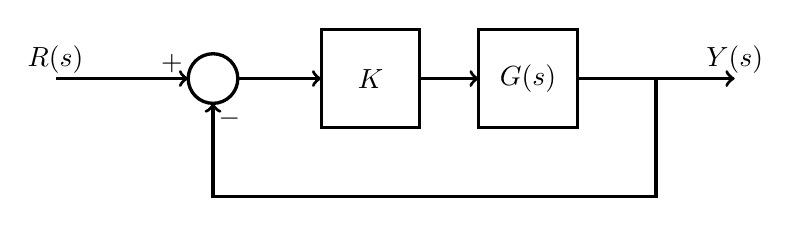
\begin{tikzpicture}[scale=1,inner sep=0pt,outer sep=0pt,very thick,
sysblock/.style={draw,rectangle,inner sep=2pt,minimum width=1.25cm,minimum height=1.25cm,inner sep=4pt, very thick}]
\draw (2,0) node[draw,circle] (sum1) {$\rule{0pt}{18pt}$};
\draw (4,0) node[sysblock] (K) {$K$};
\draw (6,0) node[sysblock] (G) {$G(s)$};
\draw[->] (0,0) node[above=2pt] {$R(s)$} -- (sum1.180) node[above left=2pt] {$+$};
\draw[->] (sum1.0)  -- (K.180);
\draw[->] (K.0) -- (G.180);
\draw[->] (G.0) -- ++(2,0) node[above=2pt] {$Y(s)$};
\draw[->] (G.0) ++(1,0) -- ++(0,-1.5) -| (sum1.-90) node[below right=2pt] {$-$};
\end{tikzpicture}
\end{center}
Suppose $G(s) = \frac{700(s+1)}{s(s+10)(s^{2}+50s+300)}$. The following is the Bode plot of $G(s)$. {\em Note that this is the Bode plot of the loop gain when $K=1$.} A control designer chooses $K=10$. What is the resulting phase and gain margin for this design? For full credit, you should indicate where you obtain information from the Bode plot to determine your answer.
\begin{center}
\includegraphics[width=5in]{\mainfolder/LectureNotes/\lecturefolder/HomeworkProblems/Problem07/bode3.pdf}
\end{center}